%%
%% This is file `sample-acmtog.tex',
%% generated with the docstrip utility.
%%
%% The original source files were:
%%
%% samples.dtx  (with options: `acmtog')
%% 
%% IMPORTANT NOTICE:
%% 
%% For the copyright see the source file.
%% 
%% Any modified versions of this file must be renamed
%% with new filenames distinct from sample-acmtog.tex.
%% 
%% For distribution of the original source see the terms
%% for copying and modification in the file samples.dtx.
%% 
%% This generated file may be distributed as long as the
%% original source files, as listed above, are part of the
%% same distribution. (The sources need not necessarily be
%% in the same archive or directory.)
%%
%%
%% Commands for TeXCount
%TC:macro \cite [option:text,text]
%TC:macro \citep [option:text,text]
%TC:macro \citet [option:text,text]
%TC:envir table 0 1
%TC:envir table* 0 1
%TC:envir tabular [ignore] word
%TC:envir displaymath 0 word
%TC:envir math 0 word
%TC:envir comment 0 0
%%
%%
%% The first command in your LaTeX source must be the \documentclass command.
\documentclass[acmtog]{acmart}
\usepackage{float}

%%
%% \BibTeX command to typeset BibTeX logo in the docs
\AtBeginDocument{%
  \providecommand\BibTeX{{%
    \normalfont B\kern-0.5em{\scshape i\kern-0.25em b}\kern-0.8em\TeX}}}

%% Rights management information.  This information is sent to you
%% when you complete the rights form.  These commands have SAMPLE
%% values in them; it is your responsibility as an author to replace
%% the commands and values with those provided to you when you
%% complete the rights form.
\setcopyright{acmcopyright}
\copyrightyear{2018}
\acmYear{2018}
\acmDOI{XXXXXXX.XXXXXXX}


%%
%% These commands are for a JOURNAL article.
\acmJournal{TOG}
\acmVolume{37}
\acmNumber{4}
\acmArticle{111}
\acmMonth{8}

%%
%% Submission ID.
%% Use this when submitting an article to a sponsored event. You'll
%% receive a unique submission ID from the organizers
%% of the event, and this ID should be used as the parameter to this command.
%%\acmSubmissionID{123-A56-BU3}

%%
%% The majority of ACM publications use numbered citations and
%% references.  The command \citestyle{authoryear} switches to the
%% "author year" style.
%%
%% If you are preparing content for an event
%% sponsored by ACM SIGGRAPH, you must use the "author year" style of
%% citations and references.
\citestyle{acmauthoryear}

%%
%% end of the preamble, start of the body of the document source.
\begin{document}

%%
%% The "title" command has an optional parameter,
%% allowing the author to define a "short title" to be used in page headers.
\title{Analysing the spatiotemporal human movement in indoor workspaces}

%%
%% The "author" command and its associated commands are used to define
%% the authors and their affiliations.
%% Of note is the shared affiliation of the first two authors, and the
%% "authornote" and "authornotemark" commands
%% used to denote shared contribution to the research.
\author{Ben Trovato}
\authornote{Both authors contributed equally to this research.}
\email{trovato@corporation.com}
\orcid{1234-5678-9012}
\author{G.K.M. Tobin}
\authornotemark[1]
\email{webmaster@marysville-ohio.com}
\affiliation{%
  \institution{Institute for Clarity in Documentation}
  \streetaddress{P.O. Box 1212}
  \city{Dublin}
  \state{Ohio}
  \country{USA}
  \postcode{43017-6221}
}

\author{Lars Th{\o}rv{\"a}ld}
\affiliation{%
  \institution{The Th{\o}rv{\"a}ld Group}
  \streetaddress{1 Th{\o}rv{\"a}ld Circle}
  \city{Hekla}
  \country{Iceland}}
\email{larst@affiliation.org}

\author{Valerie B\'eranger}
\affiliation{%
  \institution{Inria Paris-Rocquencourt}
  \city{Rocquencourt}
  \country{France}
}

\author{Aparna Patel}
\affiliation{%
 \institution{Rajiv Gandhi University}
 \streetaddress{Rono-Hills}
 \city{Doimukh}
 \state{Arunachal Pradesh}
 \country{India}}

\author{Huifen Chan}
\affiliation{%
  \institution{Tsinghua University}
  \streetaddress{30 Shuangqing Rd}
  \city{Haidian Qu}
  \state{Beijing Shi}
  \country{China}}

\author{Charles Palmer}
\affiliation{%
  \institution{Palmer Research Laboratories}
  \streetaddress{8600 Datapoint Drive}
  \city{San Antonio}
  \state{Texas}
  \country{USA}
  \postcode{78229}}
\email{cpalmer@prl.com}

\author{John Smith}
\affiliation{%
  \institution{The Th{\o}rv{\"a}ld Group}
  \streetaddress{1 Th{\o}rv{\"a}ld Circle}
  \city{Hekla}
  \country{Iceland}}
\email{jsmith@affiliation.org}

\author{Julius P. Kumquat}
\affiliation{%
  \institution{The Kumquat Consortium}
  \city{New York}
  \country{USA}}
\email{jpkumquat@consortium.net}

%%
%% By default, the full list of authors will be used in the page
%% headers. Often, this list is too long, and will overlap
%% other information printed in the page headers. This command allows
%% the author to define a more concise list
%% of authors' names for this purpose.
\renewcommand{\shortauthors}{Trovato and Tobin, et al.}

%%
%% The abstract is a short summary of the work to be presented in the
%% article.
\begin{abstract}
  Since the pandemic began in early 2020, the return to workplaces in full form has been a struggle due to the risks of the virus exposure it might create. It is recommended to avoid the use of crowded areas as much as possible. However, utilizing the office buildings and returning to normal life does not leave scope for social distancing and therefore we need a mechanism to quantify the risks of opening up workspaces to facilitate informed decision making. We analyse the movement of students and employees inside a chemistry lab and an IT office respectively to study the trajectories of human movement and spatiotemporal interactions at these workplaces. We then examine the temporary and persistent relations between human movement patterns and the workplace's overall transmission risk (based on airflow patterns) in the presence of airborne disease. Based on this analysis we present practical suggestions that can be used to minimise the risk of exposure in the workplace.
\end{abstract}

%%
%% The code below is generated by the tool at http://dl.acm.org/ccs.cfm.
%% Please copy and paste the code instead of the example below.
%%
\begin{CCSXML}
<ccs2012>
 <concept>
  <concept_id>10010520.10010553.10010562</concept_id>
  <concept_desc>Computer systems organization~Embedded systems</concept_desc>
  <concept_significance>500</concept_significance>
 </concept>
 <concept>
  <concept_id>10010520.10010575.10010755</concept_id>
  <concept_desc>Computer systems organization~Redundancy</concept_desc>
  <concept_significance>300</concept_significance>
 </concept>
 <concept>
  <concept_id>10010520.10010553.10010554</concept_id>
  <concept_desc>Computer systems organization~Robotics</concept_desc>
  <concept_significance>100</concept_significance>
 </concept>
 <concept>
  <concept_id>10003033.10003083.10003095</concept_id>
  <concept_desc>Networks~Network reliability</concept_desc>
  <concept_significance>100</concept_significance>
 </concept>
</ccs2012>
\end{CCSXML}

\ccsdesc[500]{Computer systems organization~Embedded systems}
\ccsdesc[300]{Computer systems organization~Redundancy}
\ccsdesc{Computer systems organization~Robotics}
\ccsdesc[100]{Networks~Network reliability}

%%
%% Keywords. The author(s) should pick words that accurately describe
%% the work being presented. Separate the keywords with commas.
\keywords{datasets, neural networks, gaze detection, text tagging}


%%
%% This command processes the author and affiliation and title
%% information and builds the first part of the formatted document.
\maketitle

\section{Introduction}
Reopening workplace spaces will inevitably increase contact, interaction, group gathering, and close contacts making it harder to maintain social distancing, moreover, rely on social distance for safety. This, in turn, may raise the risk of transmission inside the workplace. Changes in office layout and increased air ventilation can be useful, but the increase in exposure due to increased person-to-person contact cannot be ignored. According to the World Health Organisation (WHO), the virus that is responsible for human-human transmission may stay viable after aerosolisation in the indoor environment. As a result, while returning to the office spaces, the impacts of human mobility inside the workspace and its impact on the workplace's ability to pose minimal risk must be extensively explored.



This research seeks to model human mobility inside four distinct types of workspaces (a chemistry lab on a university campus, an IT office, a hospital ward, and a factory) while accounting for spatial density, occupancy schedules, and numerous indoor activities. Understanding the mobility of employees at a workplace will enable us to understand their behaviour and identify the day-to-day tasks they undertake as an element of work. Apart from conventional mitigation strategies such as physical distancing, improved ventilation, face masks, and personal hygiene, this will provide methods for establishing coping mechanisms to prevent exposure risk rather than treating such instances as outliers. Because this study aims to forecast human mobility inside a facility, it can be combined with various air quality index measurements to forecast transmission risk, providing numerical clarity on how crowded a workspace or point of interest within the workspace can be while still posing minimal transmission risk. Previous research in this area has focused on either understanding occupant behaviour or exploring the effect of human activities on airflow patterns in the instance of a single person model in a controlled setting. There have been a lot of studies done on leveraging Wi-Fi access point data to predict human mobility inside buildings, \cite{qian2016decimeter}, \cite{meneses2012large} but not much work has been done in-depth for discrete areas, such as a single lab or workspace. In terms of examining the impact of human mobility on indoor airflow patterns, most studies have been carried out in a planned methodology where the trajectory of the person was previously specified \cite{mahaki2021comparing}, \cite{wu2022transient}. However, the challenge is to correlate occupant behaviour with airflow patterns in the space in a non-invasive manner. We conduct a non-invasive analysis in the wild, without using a camera or any form of direct employee monitoring that can be a threat to employees' privacy, where the only data points obtained are the participants' trajectory and the air-quality index. Participants in our study were only asked to carry a Bluetooth based tag and answer a survey twice a day, their usual working behaviour or movement was not disturbed in any form. The context or labels (such as meeting schedules) of events occurring at the workplace (such as the rosters of employees working from the office) throughout the monitoring period are unknown. This adds uncertainty to the process of modelling and generalising movement behaviour, which is addressed by developing a set of uncertainty-aware rules to interpret the employee trajectories. To the best of our knowledge, this is the first work that studies the movement behaviour of occupants in an indoor office space and interweaves it with the airflow patterns in the presence of airborne disease. 

We explore the various aspects of indoor human movement throughout time and space by answering the following questions:

\begin{itemize}
    \item Do employees have a habit of visiting similar locations in the workplace?
    \item Do employees use the same routes to get from one location to another within the office?
    \item Is there a difference in the pattern of human movement during the day or between days?
    \item Is there a relationship between human movement and the density of airborne pathogens in different areas indoors?
    \item Are there any hot pockets (preferred stations, printing desk) inside the office space?
    \item Do the hot pockets get congested/crowded at regular intervals?
    \item Do the common footpaths inside the workspace pose a higher risk of transmission at all times?
    \item Do factors like sitting location, interconnecting doors, crowdedness and air quality influence human movement patterns indoors (geometric and non-geometric factors)?
\end{itemize}



Preventing the risk of infection and close contact is now part of workplace safety, posing a new challenge for sustaining workplace quality, promoting a sense of fulfilment and satisfaction, and enhancing productivity. A safer workplace will not only encourage employees to return in comfort but will also boost their performance. Because our work considers multiple kinds of workplaces, developing context-based workplace safety guidelines will serve a broader community. Therefore, the main contributions of this work are:
\begin{itemize}
    \item Event-based human-environment interaction approximation, we present an analysis of the spatiotemporal trajectories of employees inside the workspace and perform an event-based correlation between the human mobility trends and the airflow patterns inside the workspace.
    \item Spatial Context-based safety guidelines, we demonstrate practical implications of minimising the exposure risk in the presence of an airborne disease based on the relations between human movement and airflow patterns across workspaces.

\end{itemize}
The rest of this paper is organised as follows, we begin by reviewing the recent research work in this domain and identify the gaps in the literature. Then we introduce the utilised terminologies and describe the collected dataset after which we explain the methodology, elaborate on the analysis, and the results and discuss the relations between human movement and airflow patterns across workspaces before summing it up in the conclusion.


%%%%%%%%%%%%%%%%%%%%%%%%%%%%%%%%%%%%%%%%%%%%%%%%%%%%%%%%%%%%%%%%%%%%%%%%%%%%%%%%%%%%%%%%%%%%%%


\section{Related work}
With the outbreak of the pandemic and the struggle to reinstate office spaces, a lot of research has been done to reduce the risk of exposure in various types of indoor environments. Although the majority of developments in this field can be classified into three categories: safer indoor navigation, contact tracing and avoidance, and building occupancy simulation, there has also been some research to investigate the effects of human movement on air particles in an indoor space.

\subsection{Safer indoor traversal}

Minimising exposure risk in office spaces is a constant battle of avoiding crowded areas. Recent developments help cope with this by the means of path discovery techniques fit for heterogeneous environments such as university campuses and office buildings. Costa and Ge et al. introduced a graph-based indoor-outdoor path technique that examines both the exterior graph of buildings and streets and the interior graph of the entrances and exits within each building to construct a unified, context-aware path by using an on-the-fly forecasting of congestion in corridors and hallways. When tested on realistic datasets, they illustrate the efficiency of their method by demonstrating up to an order of magnitude decrease in COVID-19 exposure \cite{costa2019caprio}. Jensen and Nielsen et al. created an algorithm that can traverse both indoor and outdoor spaces and yield the true shortest path between two arbitrary points. They accomplish this by integrating different models simultaneously, where the first model maintains the distinct nature of the two spaces by having explicit connections between outdoor and indoor spaces, and the second model abstracts this distinction away, providing a unified model of outdoor-indoor space \cite{jensen2016outdoor}.


% Please add the following required packages to your document preamble:
% \usepackage{graphicx}
% \usepackage[table,xcdraw]{xcolor}
% If you use beamer only pass "xcolor=table" option, i.e. \documentclass[xcolor=table]{beamer}
\begin{table*}[!h]
\centering
\caption{Review of recent works investigating the impact of human movement on air particles in indoor spaces}
\label{tab:my-table}
\resizebox{\textwidth}{!}{%
\begin{tabular}{llllll}
\hline
{\color[HTML]{0E101A} Title} & {\color[HTML]{0E101A} Purpose} & {\color[HTML]{0E101A} Sensors used} & {\color[HTML]{0E101A} Size of dataset} & {\color[HTML]{0E101A} Models human mobility} & {\color[HTML]{0E101A} \begin{tabular}[c]{@{}l@{}}Conducted in the\\  presence of an \\ airborne disease\end{tabular}} \\ \hline
{\color[HTML]{0E101A} \begin{tabular}[c]{@{}l@{}}Occupant behaviour and\\  indoor particulate\\  concentrations in\\  daycare centres \cite{um2022occupant}\end{tabular}} & {\color[HTML]{0E101A} \begin{tabular}[c]{@{}l@{}}To analyse the effect \\ of human activity and\\  human-building \\ interaction on indoor air quality.\end{tabular}} & {\color[HTML]{0E101A} \begin{tabular}[c]{@{}l@{}}Optical particle counters, \\ real-time CO2 measurement\\ and window state data  loggers\end{tabular}} & {\color[HTML]{0E101A} Approximately 780hrs} & {\color[HTML]{0E101A} \begin{tabular}[c]{@{}l@{}}No, present a \\ discussion based \\ on scheduled activities\end{tabular}} & {\color[HTML]{0E101A} No} \\ \hline
{\color[HTML]{0E101A} \begin{tabular}[c]{@{}l@{}}Transient and continuous\\  effects of indoor human \\ movement on nanoparticle\\  concentrations in a sitting\\  person's breathing zone \cite{wu2022transient}\end{tabular}} & {\color[HTML]{0E101A} \begin{tabular}[c]{@{}l@{}}To sample the nanoparticle\\  concentration in the \\ breathing zone of a \\ sitting thermal\\  breathing manikin (STBM).\end{tabular}} & {\color[HTML]{0E101A} \begin{tabular}[c]{@{}l@{}}Sitting thermal breathing \\ manikin (STBM), Aerosol \\ generator and a medical ventilator\end{tabular}} & {\color[HTML]{0E101A} \begin{tabular}[c]{@{}l@{}}NA, controlled\\ singular experiment\end{tabular}} & {\color[HTML]{0E101A} No} & {\color[HTML]{0E101A} No} \\ \hline
{\color[HTML]{0E101A} \begin{tabular}[c]{@{}l@{}}Comparing objects for\\  human movement \\ simulation regarding\\  its air flow disturbance\\  at local exhaust ventilation \cite{mahaki2021comparing}\end{tabular}} & {\color[HTML]{0E101A} \begin{tabular}[c]{@{}l@{}}To study the disturbances\\  due to the movements \\ of a human-sized plate,\\  cylinder and detailed\\  manikin near a ventilation hood.\end{tabular}} & {\color[HTML]{0E101A} \begin{tabular}[c]{@{}l@{}}3-D sonic anemometer for\\  velocity measurements\end{tabular}} & {\color[HTML]{0E101A} \begin{tabular}[c]{@{}l@{}}NA, controlled\\ singular experiment\end{tabular}} & {\color[HTML]{0E101A} No} & {\color[HTML]{0E101A} No} \\ \hline
{\color[HTML]{0E101A} \textbf{\begin{tabular}[c]{@{}l@{}}Spatiotemporal human\\  movement in indoor\\  workspaces: A privacy\\  preserving analysis\end{tabular}}} & {\color[HTML]{0E101A} \textbf{\begin{tabular}[c]{@{}l@{}}To model the spatiotemporal \\ movement of employees \\ inside workspaces and \\ analyse their effect on\\  indoor airflow\end{tabular}}} & {\color[HTML]{0E101A} \textbf{\begin{tabular}[c]{@{}l@{}}Bluetooth tags for \\ RSSI signals and surveys\end{tabular}}} & {\color[HTML]{0E101A} \textbf{\begin{tabular}[c]{@{}l@{}}8 days for Bluetooth \\ tags, one month of survey data\end{tabular}}} & {\color[HTML]{0E101A} \textbf{Yes}} & {\color[HTML]{0E101A} \textbf{Yes}} \\ \hline
\end{tabular}%
}
\end{table*}

\subsection{Contact tracing and contact avoidance}

Contact tracing has been recognized as a crucial component of disease containment, and recent advances in this sector have fueled its efficiency by providing discoveries such as reducing the need for widespread adoption of contact tracking activities and identifying asymptotic infections. Trivedi et al. developed WiFiTrace, a network-centric approach to contact tracing that relies on passive WiFi sensing with no client-side involvement. They used WiFi network logs collected by enterprise networks for performance and security monitoring to reconstruct device trajectories for contact tracing \cite{trivedi2021wifitrace}. YYue et al. propose a neural network model termed Spatio-Temporal Episodic Memory for COVID-19 (STEMCOVID) that uses contact tracking data to detect infectious asymptotic instances. The model encodes a collective Spatio-temporal episodic memory of individuals and contains an effective parallel search mechanism based on the fusion Adaptive Resonance Theory (ART) \cite{hu2020silent}. Avoiding contact may also be accomplished by minimising congestion, which can be achieved with the help of congestion forecasting, a field that has experienced tremendous growth during the pandemic. By utilising the building floor plan and modelling human trajectory as a Gaussian distribution, Anastasiou and Costa et al created a platform for indoor congestion data generation to facilitate congestion forecasting in indoor settings. They then implemented an MCAN using this method to train congestion forecasting models in order to successfully propose pathways inside buildings while avoiding exposure to congested locations \cite{anastasiou2021epicgen}. Using game theory, Xie and Luan et al devised a crowdsourcing-based indoor navigation model that encourages users to use navigation services. They show, via simulation and theoretical analysis, that the suggested mechanism may successfully encourage responders to perform positive navigation services and acquire higher social welfare than traditional approaches \cite{xie2021game}.


\subsection{Occupancy risk estimation}
The ability of a place to provide a low-risk environment is determined by its inhabitants (number and duration of stay) as well as their interaction with the space. Sydora et al. provide a systematic simulation-based technique for calculating the infection risk for inhabitants of a building under various scenarios of building utilisation, as well as a virus transmission model that evaluates the possible infection transmission risk based on occupant behaviour \cite{sydora2022building}. Ciunkiewicz et al. devised an agent-based simulation (ABS) framework for localised settings that is highly configurable. This ABS enables extensive control over COVID-19's fast-growing epidemiological features, as well as information on risk and the impacts of both pharmaceutical and non-pharmacological interventions \cite{ciunkiewicz2022agent}. The findings of simulations can help facility administrators make better decisions and can also be utilised as inputs for a decision support system. 

\subsection{Studying indoor occupant behaviour}
The mobility of people inside a location is impacted by its physical and environmental properties. Lee et al. investigate the effects of spatial and temporal restrictions in a facility, which might limit occupants' capacity to physically remove themselves, by conducting a survey to see if and how such constraints affect occupants' physical distancing behaviours in K–12 educational facilities and the results show that spatial density influences the perceived risk of infection, the findings suggest that occupants' physical distancing behaviours are greatly influenced by crowdedness of space (i.e., spatial limitation). However, it appears that time pressure owing to limited time to meet occupancy schedules (i.e., temporal limitations) has no effect on physical distance behaviours \cite{lee2022understanding}. Jayjarah et al. developed a methodology for predicting the Likelihood of Future Non-Conformance (LFNC), which is based on the hypothesis that the likelihood of future deviations in movement behaviour is positively correlated to the intensity of trajectory deviations observed in the user's recent past and that the likelihood of future deviations increases if the user's strong-ties have also recently exhibited such non-conformant movement behaviour using longitudinal indoor location data from a university campus. They indicate that with an AUC of 0.85, the model can predict nonconformant mobility behaviour two hours in advance \cite{jayarajah2018predicting}. Chen et al. present a large-scale systematic analysis in the context of urban revisitation and re-check-in, demonstrating people's periodic behaviours and regularities by leveraging a localisation dataset to model urban revisitation and identifying features concerning POI visitation patterns, POI background information, user visitation patterns, user preference, and users. They use machine learning models to illustrate the predictive efficacy of the identified characteristics, with an overall ROC AUC of 0.92 for urban revisitation and 0.82 for re-check-in, respectively \cite{chen2020will}.



\subsection{Investigating the impact of human movement on air particles in indoor spaces}
Human activities are known to influence indoor airflow patterns, and their aerodynamic impact is dependent on characteristics such as speed, distance, and position in space. People, occupant activities, building materials, and even outside air all contribute to the effluents in indoor air. Using optical particle counters (OPS) for particulate concentration monitoring and resuspending source strengths of particles with characteristics of human-building interactions, Um et al. investigated the effects of occupant behaviour on indoor particle concentrations in daycare centres in four daycare centres in South Korea and indicate that vacuuming should be avoided while the childcare facility is inhabited by children, according to the findings. The findings also showed that opening windows without taking into account the degree of external particle concentration can drastically affect interior air quality \cite{um2022occupant}.  Wu et al. performed a series of experiments to sample the nanoparticle concentration in the breathing zone of a sitting thermal breathing manikin (STBM) in order to investigate transient variability in nanoparticle concentration. They discovered that continuous exposure to a sitting person can result in a 2.88 (1.24) percent increase in nanoparticle concentration \cite{wu2022transient}. Mahaki et al. used a human-sized plate, cylinder, and detailed manikin to study the effects of human movement on airflow patterns around local ventilation hoods both experimentally and numerically, with the movements consisting of back-and-forth movements near an exhaust hood using a 3-D sonic anemometer to measure air velocity in front of the hood opening. The results showed that the turbulence caused by the object's movements had unique air velocity peaks in the near field of the exhaust hood, which both supported and inhibited the suction flow \cite{mahaki2021comparing}.



Although some research has been done on modelling human movement for indoor environments and analysing the impact of human movement on airflow patterns inside a space, it has all been conducted in a controlled environment and thus does not take into account the spatiotemporal elements that may limit the occupant's ability to maintain a safe distance at all times or influence occupant behaviour or the day-to-day workplace habits, which may, in turn, drive the airflow pattern. Most studies consider the overall picture of the building, but what happens inside during working hours or scheduled activities, and its impact on controlling or lowering the risk of infection, are yet unknown. There are broad rules for personal hygiene and social distance, but in a space that is used by a variety of individuals throughout the day, as well as visitors and passers-by, the assumption that "if everyone does their bit, we'll all be safe" may not be sufficient.
Therefore the following gaps exist in the literature:
\begin{itemize}
    \item Lack of understanding about the spatiotemporal human movement inside different kinds of workspaces.
    \item Lack of a framework that correlates the indoor airflow pattern of a workspace with their respective human movement trends.
    \item Lack of understanding of the practical implications of the relations between human movement and airflow patterns across workspaces.
\end{itemize}


%%%%%%%%%%%%%%%%%%%%%%%%%%%%%%%%%%%%%%%%%%%%%%%%%%%%%%%%%%%%%%%%%%%%%%%%%%%%%%%%%%%%%%%%%%%%%%


\section{Data Collection}
The research was carried out at four locations, including a chemical wet lab at RMIT University, an IT workplace, a Covid-19 ward within a hospital, and a factory, and the data collection process was authorised by our university's Human Research Ethics Committee. The timeframe of data collection varied per site, and data was collected in two forms: participant trajectories using BLE tags and a survey.

\subsection{Participants}
Each site has its own set of participants. Each site's employees/students were briefed regarding the study and the data collection process. Those who volunteered to participate in the research were asked to fill out and sign consent forms, which were collected and held in a locked box to safeguard the participants' privacy. Details about the consent form...volunteers could discontinue at any time... After participants returned the completed consent forms, they were asked to wear a Bluetooth tag while they were in the workspace, during the research. Participants were requested to wear the same tag for the duration of the study. There was no participant information associated with the tag. Every day, the participants were also asked to complete a 15-question survey. Participants were required to provide their email address in order to register for daily survey reminders, but their email address was not linked to any other information and was only used to deliver survey reminders. The survey also did not collect any personal information.

\subsection{Collected Data}
\subsubsection{Movement Data}
Participants were requested to carry Kontakt Asset Tag-2(s) in their pockets for the duration of the study in order to record their mobility in their workspaces. Participants were requested to wear the same tag for the course of the research, but no information about the participant connected with the tag was recorded. Kontakt Asset Tag-2 Bluetooth tags are equipped with a 3DH motion sensor and are capable of over-the-air communication using Bluetooth over a range of up to 50m. Gateways detect and collect the BLE signals sent by these tags. These signals were received using Kontakt portal lights, which are plug-and-play BLE gateways. The Asset Tag-2 also has an infrared receiver, which, when paired with the gateway light, can offer room-level location precision. The portal lights can connect to an existing Wi-Fi network and have a Bluetooth range of 50 metres. Their working mechanism is as follows:
The Asset Tag-2 are transmitters with a unique identification code that they communicate using Bluetooth Low Energy technology to surrounding receivers, which in this case are the Kontakt portal lights. The unique Asset Tag identification (i.e. tracking id) that is broadcast can be used to determine the presence and movement of a person carrying a certain tag. A gateway device passively monitors its surroundings for BLE card beacons. When beacons are detected, the gateway continually gathers beacon data such as their unique IDs, start and end timestamps, and RSSI. RSSI is used by the gateway to assess the proximity of the beacons to the gateway. Every 1.5 seconds, gateways send the collected beacon data to the cloud storage server. 
\begin{figure}[h]
  \centering
  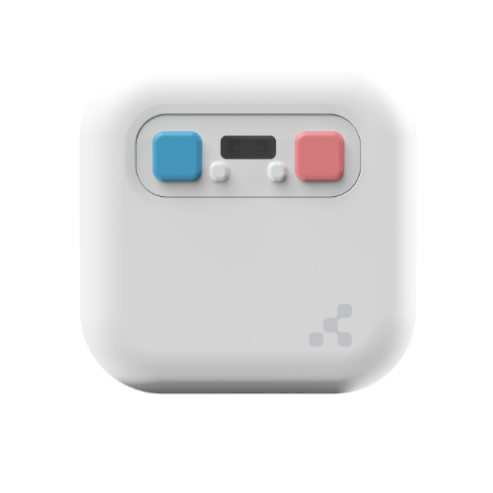
\includegraphics[width=3cm,height=3cm,keepaspectratio]{Asset-Tag-493x0-c-default}
  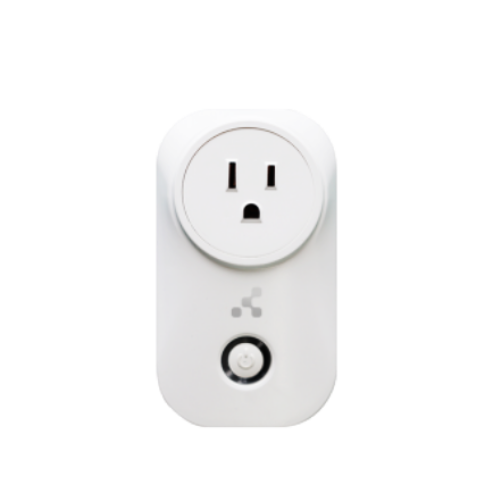
\includegraphics[width=4cm,height=4cm,keepaspectratio]{Group-15446-493x0-c-default}
  \caption{Kontakt Asset Tag-2 and Gateway}
  \end{figure}
The data acquired by the gateways was available through the Kontakt REST and Streams API in two formats: location, occupancy, telemetry, and sensor data as processed JSON in the form of a GET request or as raw RSSI signals. For each tag, JSON replies were provided once every minute, but RSSI signals were available every five seconds. We used RSSI signals for this experiment.

\subsubsection{Survey Data}
For the duration of the study, participants were asked to complete a 15-question survey twice daily (if they were working from the office). This survey was designed to capture the ground truth about the participants' mobility patterns in the workplace. It included questions regarding the participant's seating location, their most-used pathway inside the workspace, interactions with coworkers, whether or not they interacted with others around them, trips away from the workstation, noise, and concentration levels. There was also a question about whether or not the participants were wearing masks. Participants were also encouraged to include their Asset tag ID in the survey response so that mobility data and survey results could be compared. To protect participant privacy, the survey included no personal information, and hence the Asset tag ID could not be used to retrace the participant.

\subsection{Procedure}
Before collecting data, all Asset tags were synchronised and configured to a level 2 (possible values were 1-5) of signal transmission that emits up to a range of 10m since it provided the best location accuracy for our experimental setup. The advertisement rate was set to 100 milliseconds. The gateways were configured with the default settings, and a separate Wi-Fi network was set up for them. 
\begin{figure}[h]
  \centering
  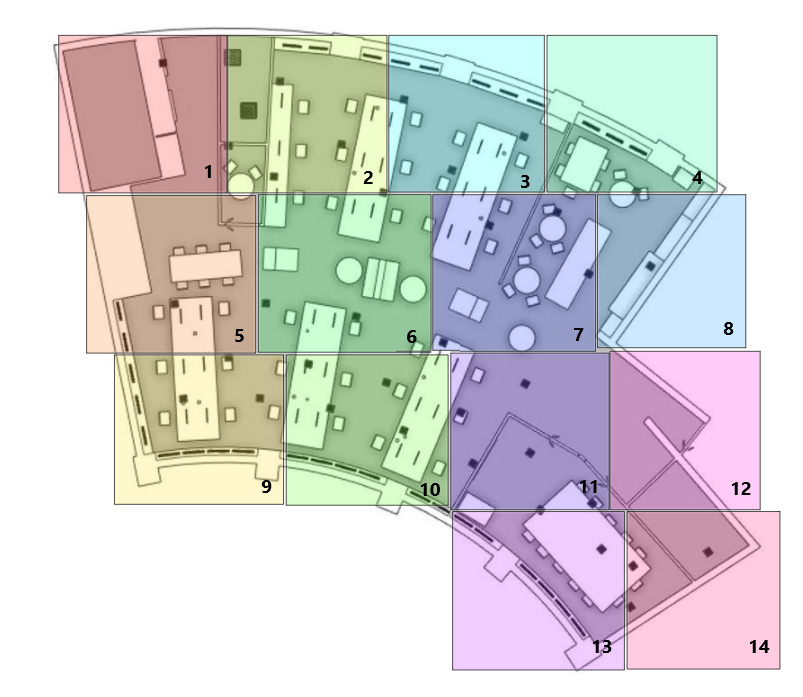
\includegraphics[width=4cm,height=4cm,keepaspectratio]{grids.png}
  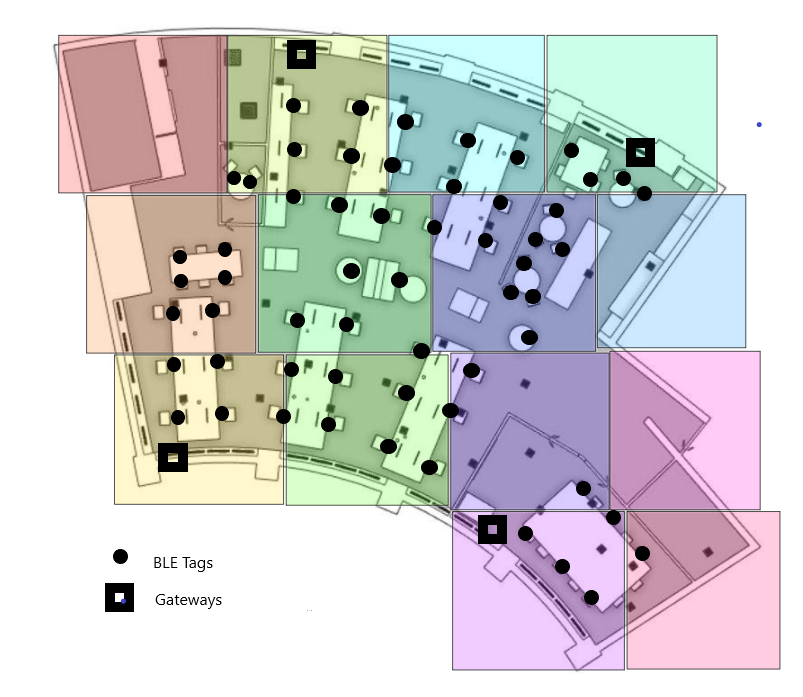
\includegraphics[width=4cm,height=4cm,keepaspectratio]{sensors_grids.png}
  \caption{Workspace divided into 14 grids (left) and the stationary tags deployed for fingerprinting along with the gateways (right)}
  \label{Memkogrids}
  \end{figure}
The workplace area was split into 14 equal-sized grids for the purpose of the experiment, as illustrated in Figure-\ref{Memkogrids} (left). Grids encompass workstations, meeting and conference rooms, a kitchen area, and the printing station. Then we performed a fingerprinting experiment, which was eventually used to train the localisation model. To accomplish the fingerprinting, we placed 4-5 Asset Tags in each grid for two days to simulate the presence of employees. As illustrated in Figure-\ref{Memkogrids} (right), there were 65 stationary tags and four gateways deployed within the office space. We collected 2000 continuous data points per tag and trained the localisation model in the following manner. We chose a 20-second duration (the 30-second duration was also used, but the accuracy was better with the 20-second duration) to segment the continuous data points proportionally, and then extracted statistical features such as the minimum, maximum, mean, median, variance, first quartile, and third quartile. We also had the timestamps and occupancy labels (grid IDs) of the stationary tags, which we segmented over the same time period. This resulted in a dataset simulating employees in the workplace, complete with RSSI characteristics and tagged occupancy levels, which we used to forecast employee movements. We trained three classification models, namely Support Vector Machine (SVM), Logistic Regression, and K-Nearest Neighbor (n=5), and assessed their performance on the test set (20\% of the data was utilised for testing), with K nearest neighbour achieving the highest reporting accuracy of 90\%. The prediction accuracy was computed by dividing the number of correctly predicted instances by the total number of instances assessed. We acknowledge that the stationary tags may not accurately represent employee movement within the workspace, but since it was not feasible to carry out a fingerprinting experiment by moving around the office during working hours, we placed multiple tags in each grid to generate a sense of the various locations the employees may be present at.
\begin{itemize}
    \item Following the establishment of the localisation model, participants were encouraged to take an Asset Tag each; we had 13 participants for a period of 6 days and gathered 12,000 trajectories for each participant.
    \item The survey was sent out on all working days at 11:00 AM and 16:00 PM, and we received an average of 8 responses each day, and a total of 173 responses. Approximately 40\% of the workers who work from the office volunteered to take part in the survey.
    \item Participants were asked to return the Asset Tags in the allocated box at the completion of the data collection period.
\end{itemize}

%%%%%%%%%%%%%%%%%%%%%%%%%%%%%%%%%%%%%%%%%%%%%%%%%%%%%%%%%%%%%%%%%%%%%%%%%%%%%%%%%%%%%%%%%%%%%%


\section{Terminologies}
Here we define the various terminologies for the context of our analysis. 
\begin{itemize}
    \item Human movement: The term "human movement" refers to the movement of employees across grids for the sake of this research, taking into account the presence of numerous persons in a single grid as well as one or more employees travelling across various grids at the same time. This research does not take into consideration an employee's mobility inside a grid.
    \item Dwell location: The dwell location for each employee for this analysis has been taken as the grid where the employee spends maximum time, on most days, the value of which is the ID of that grid. It should be noted that the exact dwell location of the employee cannot be estimated from this experiment. However, in some cases when the participant mentioned their Asset Tag ID in the survey, their dwell locations can be compared to assess the validity of this method.
    \item Trajectory: An instance of an employee present in the workspace where their location can be estimated within the workspace is considered as its trajectory for this study. For example an employee present in grid 2 for 10 minutes; and an employee moving from grid 2 to grid 5 to grid 10 in the last 2 minutes.
  
\end{itemize}


%%%%%%%%%%%%%%%%%%%%%%%%%%%%%%%%%%%%%%%%%%%%%%%%%%%%%%%%%%%%%%%%%%%%%%%%%%%%%%%%%%%%%%%%%%%%%%


\section{Data preprocessing}
The data cleaning procedure was carried out in two parts, the first cleaning instances in the raw RSSI data when the tag could not be recognised by all four gateways, resulting in RSSI values of 0 for some gateways. This might be due to a network technical fault or the tag being out of reach for one or more gateways. The best available values were utilised in this circumstance. The second stage is to clean the predicted employee trajectories because the prediction model was only trained for two days using stationary tags and forecasted the employee hopping over numerous grids in a relatively short period of time.  
The resulting dataset comprised timestamps, Asset Tag IDs, and grid-IDs after the localisation model predicted the locations of the employees. Features such as previous grid-ID, next grid ID, grid change status, and time spent in the grid were calculated using data frame manipulation techniques from Python's pandas module. When the trajectories of employees were examined, it was discovered that the dataset had a substantial level of noise. As a result, the following criteria were used to clean the data.
  
\begin{itemize}
    \item There were multiple instances where the users' location was picked up as a nearby grid, just once every few minutes for a period shorter than 20 seconds. Because these hops were quite short in duration and were redundant throughout the data, all such instances were labelled as the user's dwell location using the following formula: 
    If the time spent in a grid is less than 0.33 minutes, 
    and previous and next grid locations are the same,
    And the current grid is a nearby grid of dwell grid, 
    then current grid = dwell location.	
    \item In certain cases, the employee was seated on the boundary of two grids, prompting the model to frequently forecast the person's presence in the other grid. This was a pattern throughout all employee trajectories where there was at least one neighbouring grid that had been predicted as the location, and travel to and from that grid was random and redundant over all days and hours of the day. As a result, using the following rule, this pseudo-location was recognised and labelled as each employee's dwell location:
    if there are a lot of employee trajectories back and forth from a neighbouring grid, 
    and there are no other grids visited in between, 
    the trajectories of the neighbouring grid = the seating location.    
    \item The noise was noticed not just in cases when the employee was present at their seating position, but also when the user was not present at their seating location. As a result, if the employee's trajectory showed frequent hops between two neighbouring grids, they were combined into the grid the user was originally at or spent more time at using the clause: 
    If time spent in a grid is less than 0.33 minutes,
    And previous and next grid locations are the same,
    And the current grid is a nearby grid of the previous/next grid,
    then current grid = previous/next location.
\end{itemize}


We acknowledge that we do not have any ground truth behind these rules used for noise removal but they were carefully devised by taking into consideration the presence of common patterns across all days or each hour of the day and sometimes for every user.


%%%%%%%%%%%%%%%%%%%%%%%%%%%%%%%%%%%%%%%%%%%%%%%%%%%%%%%%%%%%%%%%%%%%%%%%%%%%%%%%%%%%%%%%%%%%%%

\section{Methodology}

Modifying the template --- including but not limited to: adjusting
margins, typeface sizes, line spacing, paragraph and list definitions,
and the use of the \verb|\vspace| command to manually adjust the
vertical spacing between elements of your work --- is not allowed.






\section{Analysis of workspace behaviour}
Out of 13 participants, 7 volunteered to enter their Asset Tag IDs in the survey responses, which served as ground truth for our analysis methodology. After data cleaning, for every participant, we identified the grids where they spend maximum time (continuous) and labelled them as their dwell location. We verified our approach by comparing these locations with the dwell locations mentioned in the survey responses for which we achieved 100% accuracy. After this, we analysed the employee trajectories to understand the locations they visit, the paths they take to visit them and the amount of time they spend at these locations. We identified three locations for each employee and the paths they take to get to these three locations and compared them to the "frequent walking paths" mentioned in the survey response. 

The employees have a habit of using the same paths to visit the same locations. 

Thereafter we identified the most used grids in the workspace and the purpose of their usage, the number of employees that are present in these grids at a time and the duration of their stay. Grids 3, 5, 7, 1 and 10 are the grids where maximum activity is observed and these are the common frequent locations across all participants. Grid 1 remains a popular destination for employees throughout the day which is not surprising as it gets utilised during restroom breaks and there is only one printing station in the office which is situated in this grid. The activity in grid 7 follows a trend. It starts getting busy after 11 AM, gets the busiest between 12:00 PM -13:00 and sees a decrease in human movement after 14:00. It can house up to 9 employees in an hour and they usually spend anywhere between approximately 2 to 20 minutes in the kitchen space during a single visit. It should be noted that grid 7 also covers the walking path that connects the kitchen area to the workstations and hence receives walking activity too. The activity in grid 5 also remains consistent throughout the day as employees utilise the grid to reach the restroom and the printing station in grid 1. It contains two workstations, and a common table apart from the part of the walking track for people sitting in grid 9. Employees generally spend between 30 seconds to 2 minutes here.  The popularity of grids 4 and 11 is similar and that of 2, 6, as well as that of grids 8 and 9. Grid 4 sees the presence of one or two employees around lunchtime and does not receive much activity apart from this. This could be because it contains the far-off part of the sitting area inside the kitchen space and may be an unpopular choice of dwelling for having lunch. The human movement in grid 6 also stays consistent throughout the day, where employees spend between 2 and 3 minutes during each stay, owing to its central location and versatile geometry covering six workstations, a coffee table, a couch as well as a common walking path for anyone travelling to the other half of the workspace. The number of time people spend in the kitchen grid 8, do they turn on an appliance, go back and then come back when their food is ready?

It should be noted that there are two meeting rooms present in the study area, one with a capacity of 20 people and the other with a capacity of two. The bigger meeting room (grid 13 and 14) does not seem to be utilised for group meetings as per the trajectories since none of the participants spend longer than 3 minutes in the meeting room and at any given time, multiple people were not spotted to be inside the meeting room. It also forms one of the least popular locations inside the workspace. We validated this observation by examining the trends of CO2 levels, the TVOCs and the suspended particles in the meeting room which revealed that they are consistent and do not show any major events of deviation from the usual pattern. However, the trajectories suggest that employees may have utilised the part of the meeting room covered by grid 11 to take individual calls as higher noise was observed in the presence of a single participant for a period of approximately 20 minutes.

This was true for all six days of the study. 10:30 to 1:30 on 21, two people in grid 13. 

We recommend spacing out the meetings or leaving the meeting room for a few minutes after each meeting.

Every employee visits a set of locations each day during their stay at the workplace. These are the kitchen area, the restroom, the meeting room(s) as well as a place to interact with their colleagues. 


\section{Results and Discussion}



\section{Authors and Affiliations}



\section{Rights Information}



\section{CCS Concepts and User-Defined Keywords}

Two elements of the ``acmart'' document class provide powerful
taxonomic tools for you to help readers find your work in an online
search.

The ACM Computing Classification System ---
\url{https://www.acm.org/publications/class-2012} --- is a set of
classifiers and concepts that describe the computing
discipline. Authors can select entries from this classification
system, via \url{https://dl.acm.org/ccs/ccs.cfm}, and generate the
commands to be included in the \LaTeX\ source.

User-defined keywords are a comma-separated list of words and phrases
of the authors' choosing, providing a more flexible way of describing
the research being presented.

CCS concepts and user-defined keywords are required for for all
articles over two pages in length, and are optional for one- and
two-page articles (or abstracts).

\section{Sectioning Commands}

Your work should use standard \LaTeX\ sectioning commands:
\verb|section|, \verb|subsection|, \verb|subsubsection|, and
\verb|paragraph|. They should be numbered; do not remove the numbering
from the commands.

Simulating a sectioning command by setting the first word or words of
a paragraph in boldface or italicized text is {\bfseries not allowed.}

\section{Tables}




%%
%% The acknowledgments section is defined using the "acks" environment
%% (and NOT an unnumbered section). This ensures the proper
%% identification of the section in the article metadata, and the
%% consistent spelling of the heading.
\begin{acks}
To Robert, for the bagels and explaining CMYK and color spaces.
\end{acks}

%%
%% The next two lines define the bibliography style to be used, and
%% the bibliography file.
\bibliographystyle{ACM-Reference-Format}
\bibliography{base}

%%
%% If your work has an appendix, this is the place to put it.
\appendix



\end{document}
\endinput
%%
%% End of file `sample-acmtog.tex'.
